%%%%%%%%%%%%%%%%%%%%%%%%%%%%%%%%%%%%%%%%%%%%%%%%%%%%%%%%%%%%%%%%%%%%%%
% writeLaTeX Example: Academic Paper Template
%
% Source: http://www.writelatex.com
% 
% Feel free to distribute this example, but please keep the referral
% to writelatex.com
% 
%%%%%%%%%%%%%%%%%%%%%%%%%%%%%%%%%%%%%%%%%%%%%%%%%%%%%%%%%%%%%%%%%%%%%%
% How to use writeLaTeX: 
%
% You edit the source code here on the left, and the preview on the
% right shows you the result within a few seconds.
%
% Bookmark this page and share the URL with your co-authors. They can
% edit at the same time!
%
% You can upload figures, bibliographies, custom classes and
% styles using the files menu.
%
% If you're new to LaTeX, the wikibook is a great place to start:
% http://en.wikibooks.org/wiki/LaTeX
%
%%%%%%%%%%%%%%%%%%%%%%%%%%%%%%%%%%%%%%%%%%%%%%%%%%%%%%%%%%%%%%%%%%%%%%
\documentclass[twocolumn,showpacs,%
  nofootinbib,aps,superscriptaddress,%
  eqsecnum,prd,notitlepage,showkeys,10pt]{revtex4-1} % chktex 8

% \usepackage{biblatex}
% \addbibresource{Report/referencias.bib}
% \addbibresource{Report/mainNotes.bib}

\usepackage[portuguese]{babel}
\usepackage[shortlabels]{enumitem}
\usepackage[utf8]{inputenc}
\usepackage{amssymb}
\usepackage{amsmath}
\usepackage{graphicx}
\usepackage{dcolumn}
\usepackage{xcolor}
\usepackage[pdfstartview=FitH,
            colorlinks,
            bookmarksnumbered,
            bookmarksopen,
            linktocpage,
            urlcolor=blue,
            linkcolor=red!70!black,
            citecolor=red!70!black]{hyperref}
\usepackage{float}
% \usepackage{multicol}
\usepackage{listings}
\usepackage{xfrac}
\usepackage{color}
\usepackage{tikz}
\usetikzlibrary{shapes, arrows}

\tikzstyle{terminator} = [rectangle, draw, text centered, rounded corners, minimum height=2em]
\tikzstyle{process} = [rectangle, draw, text centered, minimum height=2em]
\tikzstyle{decision} = [diamond, draw, text centered, minimum height=2em]
\tikzstyle{data}=[trapezium, draw, text centered, trapezium left angle=60, trapezium right angle=120, minimum height=2em]
\tikzstyle{connector} = [draw, -latex']

\definecolor{dkgreen}{rgb}{0,0.6,0}
\definecolor{gray}{rgb}{0.5,0.5,0.5}
\definecolor{mauve}{rgb}{0.58,0,0.82}

\lstset{frame=tb,
  language=[90]Fortran,
  aboveskip=3mm,
  belowskip=3mm,
  showstringspaces=false,
  columns=flexible,
  basicstyle={\small\ttfamily},
  numbers=none,
  numberstyle=\tiny\color{gray},
  keywordstyle=\color{blue},
  commentstyle=\color{dkgreen},
  stringstyle=\color{mauve},
  breaklines=true,
  breakatwhitespace=true,
  tabsize=4
}

\usepackage{booktabs}
\setlength{\heavyrulewidth}{1.5pt}
\setlength{\abovetopsep}{4pt}

\usepackage[nottoc,numbib]{tocbibind}
\usepackage{physics}

\usepackage[cmintegrals,cmbraces]{newtxmath}
\usepackage{ebgaramond-maths}

\newcommand{\C}{\mathbb{C}}
\newcommand{\R}{\mathbb{R}}
\newcommand{\N}{\mathbb{N}}
\newcommand{\Z}{\mathbb{Z}}

\DeclareMathOperator\erfc{erfc}
\newcommand*\diff{\mathop{}\!\mathrm{d}}
\newcommand*\Diff[1]{\mathop{}\!\mathrm{d^#1}}
\renewcommand{\leq}{\leqslant}
\renewcommand{\geq}{\geqslant}
\newcommand* \e{\mathrm{e}}

\makeatletter
  \DeclareSymbolFont{ntxletters}{OML}{ntxmi}{m}{it}
  \SetSymbolFont{ntxletters}{bold}{OML}{ntxmi}{b}{it}
  \re@DeclareMathSymbol{\leftharpoonup}{\mathrel}{ntxletters}{"28} % chktex 18
  \re@DeclareMathSymbol{\leftharpoondown}{\mathrel}{ntxletters}{"29} % chktex 18
  \re@DeclareMathSymbol{\rightharpoonup}{\mathrel}{ntxletters}{"2A} % chktex 18
  \re@DeclareMathSymbol{\rightharpoondown}{\mathrel}{ntxletters}{"2B} % chktex 18
  \re@DeclareMathSymbol{\triangleleft}{\mathbin}{ntxletters}{"2F} % chktex 18
  \re@DeclareMathSymbol{\triangleright}{\mathbin}{ntxletters}{"2E} % chktex 18
  \re@DeclareMathSymbol{\partial}{\mathord}{ntxletters}{"40} % chktex 18
  \re@DeclareMathSymbol{\flat}{\mathord}{ntxletters}{"5B} % chktex 18
  \re@DeclareMathSymbol{\natural}{\mathord}{ntxletters}{"5C} % chktex 18
  \re@DeclareMathSymbol{\star}{\mathbin}{ntxletters}{"3F} % chktex 18
  \re@DeclareMathSymbol{\smile}{\mathrel}{ntxletters}{"5E} % chktex 18
  \re@DeclareMathSymbol{\frown}{\mathrel}{ntxletters}{"5F} % chktex 18
  \re@DeclareMathSymbol{\sharp}{\mathord}{ntxletters}{"5D} % chktex 18
  \re@DeclareMathAccent{\vec}{\mathord}{ntxletters}{"7E} % chktex 18
\makeatother

\DeclareMathAlphabet\mathbfcal{OMS}{cmsy}{b}{n}

\begin{document}

\title{
  Equação do calor e o problema da adega
}
\author{Caio Tomás de Paula}
\affiliation{Departamento de Matemática, Universidade de Brasília, Brasil.}
%
\begin{abstract}
    Relatório entregue como parte do trabalho final do curso de Introdução a
    Métodos Computacionais em Equações Diferenciais Parciais (IMCEDP) do
    Programa de Pós-Graduação em Matemática (PPGMAT),
    ministrado pelo prof. Dr.~Yuri Dumaresq Sobral no segundo semestre letivo
    de 2023 da Universidade de Brasília.
    O objetivo do trabalho foi resolver, numericamente, a equação do calor.
    Foi utilizada~\cite{lin1998} como referência principal para o trabalho, além
    das notas de aula do curso e do livro~\cite{Iserles}.
\end{abstract}
%
\maketitle
%
\section{Introdução}
%
	Estamos interessados em estudar a variação da temperatura do solo terrestre a uma dada
	profundidade $x$ no instante $t$. Desconsiderando a curvatura da terra e a variação diária
	de temperatura da superfície, podemos modelar a distribuição de temperatura $u(x,t)$ à
	profundidade $x$ no tempo $t$ por uma equação do calor unidimensional:
	%
	\begin{equation*}
		u_t = \kappa u_{xx}.
	\end{equation*}
	%
	A difusividade térmica do solo terrestre será considerada $\kappa = 6.3\text{m}^2/\text{ano}$.
	Note que estamos desconsiderando o calor oriundo do núcleo da Terra, já que não há forçamento
	na equação. Vamos assumir que $u \xrightarrow{x\to\infty} 0$. Vamos também assumir que
	a temperatura $f(t)$ na superfície ($x = 0$) assume apenas dois valores: uma temperatura
	de ``verão'' durante metade do ano e uma temperatura de ``inverno'' durante a outra metade.
	Esse padrão se repete todo ano, i.e., a temperatura é periódica em $x=0$ com período de 1 ano.

	Em símbolos,
	%
	\begin{equation*}
		f(t) = \begin{cases}
			T_s, \ 0 \leq t < 1/2 \\
			T_w, \ 1/2 \leq t \leq 1,
		\end{cases}
	\end{equation*}
	%
	onde $T_s$ denota a temperatura no verão e $T_w$ denota a temperatura no inverno, com $t$ em anos.

	Vamos tomar a condição inicial $u(x,0) = f(t)\e^{-q_1x}$, com $q_1 = 0.71\text{m}^{-1}$.
	Por fim, vamos tomar $u(L,t) = 0$, com $L$ suficientemente longo para que essa condição seja
	válida.

	Em resumo, queremos resolver o PVIC
	%
	\begin{equation*}
		\begin{cases}
			u_t = \kappa u_{xx}, \ 0 \leq x \leq L, t\geq 0 \\
			u(x,0) = f(t)\e^{-q_1x} \\
			u(0,t) = f(t) \\
			u(L,t) = 0
		\end{cases}
	\end{equation*}
	%

	Queremos resolver este problema numericamente e responder a algumas perguntas.
	Mais especificamente, vamos resolver este problema usando tanto o método de Euler
	explícito (e mostrar sua ordem) quanto o método de Crank-Nicolson, encontrar
	a profundidade ideal para uma adega de vinhos e resolver uma variação
	do problema com difusividade variável.
%
\section{Uma análise teórica}
%
	Antes de partir para a solução numérica, vamos fazer algumas considerações sobre
	a solução analítica do problema. Primeiro, note que podemos escrever
	%
	\begin{equation}
		f(t) = \sum_{n=-\infty}^{\infty} c_n \e^{2\pi int/T},
	\end{equation}
	%
	com $C_n\in\mathbb{C}$ tais que $\overline{C_n} = C_{-n}$ e $T = 1$ ano.
	É possível mostrar\footnote{~\cite[p.~129]{lin1998}} que, em um tempo $t$,
	uma substância se difunde aproximadamente $\sqrt{\kappa t}$ unidades.
	Sendo assim, na escala de tempo de interesse (1 ano), temos
	%
	\begin{equation}
		\sqrt{\kappa T} = \sqrt{6.3} \approx 2.5\text{ m}.
	\end{equation}
	%
	Vamos tomar o \textit{ansatz}
	%
	\begin{equation}
		u(x,t) = \sum_{n=-\infty}^{\infty} C_n \omega_n(x) \e^{2\pi int/T},
	\end{equation}
	%
	com $C_n\in\mathbb{C}$ tais que $\overline{C_n} = C_{-n}$, de modo que $u$ é real.
	Vamos impor as seguintes condições:
	%
	\begin{itemize}[(i)]
		\item cada uma das parcelas satisfaz a equação do calor
		\item $\omega_n(0) \equiv 1$, de modo que a representação de $f(t)$ seja recuperada
		\item $\omega_n(x)$ é limitado e tende a 0 quando $x\to\infty$ ($n\neq 0$),
		uma vez que a temperatura a profundidades muito grandes não é sensível a variações
		de temperatura na superfície.
	\end{itemize}
	%
	A condição (i) nos dá
	%
	\begin{equation}
		\frac{\diff^2\omega_n}{\diff x^2} = p^{2}_n\omega_n, \ p^{2}_n = \frac{2\pi i n}{\kappa T}.
	\end{equation}
	%
	Consequentemente,
	%
	\begin{equation}
		p_n = \pm(1 \pm i)q_n, \ \text{ com } \ q_n = \sqrt{ \frac{|n|\pi}{\kappa T} } > 0
	\end{equation}
	%
	e o sinal $\pm$ depende do sinal de $n$. Desta forma, a solução geral da EDO de $\omega_n$
	é dada por
	%
	\begin{equation}
		\omega_n(x) = A_n\e^{(1 \pm i)q_n x} + B_n\e^{-(1 \pm i)q_n x}.
	\end{equation}
	%
	Da condição (iii) segue que $A_n \equiv 0$ e da condição (ii) segue que
	$B_n \equiv 1$. Portanto, obtemos
	%
	\begin{equation}
		\omega_n(x) = \e^{-(1 \pm i)q_n x}
	\end{equation}
	%
	e, assim,
	%
	\begin{equation}
		u(x,t) = \sum_{n=-\infty}^{\infty} C_n \e^{-(1 \pm i)q_n x} \e^{2\pi int/T}.
	\end{equation}
	%
	Escrevendo $C_n = |C_n|\e^{-i\gamma_n}$, segue que
	%
	\begin{equation}
		u(x,t) = C_0 + 2\sum_{n=1}^{\infty} |C_n| \e^{-q_n x}\cos\left( \frac{2\pi nt}{T} + \gamma_n - q_n x \right).
	\end{equation}
	%
	Vamos interpretar esta solução. Note que o termo do cosseno representa uma onda de frequência
	$2\pi n/T$ e número de onda $q_n$. Por conta disto, a $n$-ésima ``onda parcial'' se propaga
	com velocidade
	%
	\begin{equation}
		\frac{2\pi n}{q_n T} = \sqrt{ \frac{ 4\pi\kappa|n| }{T} }.
	\end{equation}
	%
	Como há um amortecimento exponencial na direção de propagação e este amortecimento
	cresce com $\sqrt{|n|}$, segue que a contribuição mais importante para a solução
	vem do termo com $n=1$. Para os valores numéricos que estamos considerando,
	segue que
	%
	\begin{equation}
		q_1 = \frac{1}{2\pi}\sqrt{\frac{4\pi\kappa}{T}} \approx 0.71\text{m}^{-1}.
	\end{equation}
	%
	Agora, note que o ponto $x_1$ tal que $q_1x_1 = \pi$ é tal que a temperatura
	$u(x_1,t)$ é oposta em fase à temperatura $u(0,t)$. Dito de outro modo,
	$x_1 = \pi/q_1 \approx 4.4$m é a profundidade na qual a temperatura do solo
	tem fase oposta à temperatura da superfície. Isto significa que se na superfície
	a temperatura é de verão então à profundidade $x_1$ a temperatura é de inverno.
	Além disso, a variação de temperatura é $\e^{-\pi} \approx 4\%$ da variação na superfície.
	Isto torna esta profundidade ideal para uma adega de vinhos!
%
\section{Métodos numéricos}
%

	Começamos resolvendo a equação com o método de Euler explícito,
	%
	\begin{equation}
		u^{n+1}_{\ell} = u^{n}_{\ell} + \mu( u^{n}_{\ell + 1} - 2u^{n}_{\ell} + u^{n}_{\ell - 1} ),
	\end{equation}
	%
	que converge
	para $\kappa\mu \leq 1/2$. Por conta desta restrição ao número de Courant,
	não podemos escolher $\Delta t$ e $\Delta x$ de forma displicente.

	Também utilizamos o método de Crank-Nicolson para resolver o problema.
	Este método, dado por
	%
	\begin{equation}
		\label{eq:crank-nicolson}
		-\alpha u^{n+1}_{\ell + 1} + (1 + 2\alpha)u^{n+1}_{\ell} - \alpha u^{n+1}_{\ell - 1}
		= \alpha u^{n}_{\ell + 1} + (1 - 2\alpha)u^{n}_{\ell} + \alpha u^{n}_{\ell - 1}
	\end{equation}
	%
	com $\alpha = \kappa\mu/2$ é implícito, incondicionalmente estável e consistente
	(logo convergente pelo Teorema de Equivalência de Lax).
	Consequentemente, temos maior liberdade na escolha de $\Delta t$ e $\Delta x$, o que torna
	este método mais indicado para o cômputo da solução por grandes intervalos de tempo.
	A implicitude do método nos obriga a resolver um sistema linear a cada iteração,
	dado por
	\begin{equation}
		\begin{bmatrix}
			1 + 2\alpha & -\alpha & 0 & \cdots & 0 \\
			-\alpha & 1 + 2\alpha & -\alpha & \ddots & \vdots \\
			0 & -\alpha & 1 + 2\alpha & \ddots & 0 \\
			\vdots & \ddots & \ddots & \ddots & -\alpha \\
			0 & \cdots & 0 & -\alpha & 1 + 2\alpha
		\end{bmatrix}
		\begin{bmatrix}
			u_1 \\
			u_2 \\
			u_3 \\
			\vdots \\
			u_{N-1} \\
			u_N
		\end{bmatrix}
		=
		\begin{bmatrix}
			b_1 \\
			b_2 \\
			b_3 \\
			\vdots \\
			b_{N-1} \\
			b_N
		\end{bmatrix},
	\end{equation}
	sendo $N$ a quantidade de pontos na malha espacial.
	Para resolver tal sistema, usamos o \href{https://en.wikipedia.org/wiki/Tridiagonal_matrix_algorithm}{algoritmo da matriz tridiagonal}
	(ou de Thomas).
%
\section{Resultados}
%
	Começamos resolvendo a equação utilizando o método de Euler explícito.
	Tomamos um intervalo espacial de 0m a 15m e um intervalo temporal de 0 a 1 ano.
	Os valores de $\Delta x$ e $\Delta t$ foram tomados de maneira que $\kappa\mu \leq 1/2$
	para que o método convergisse.
	%
	\begin{figure}[t]%
		\label{fig:exp-euler}
		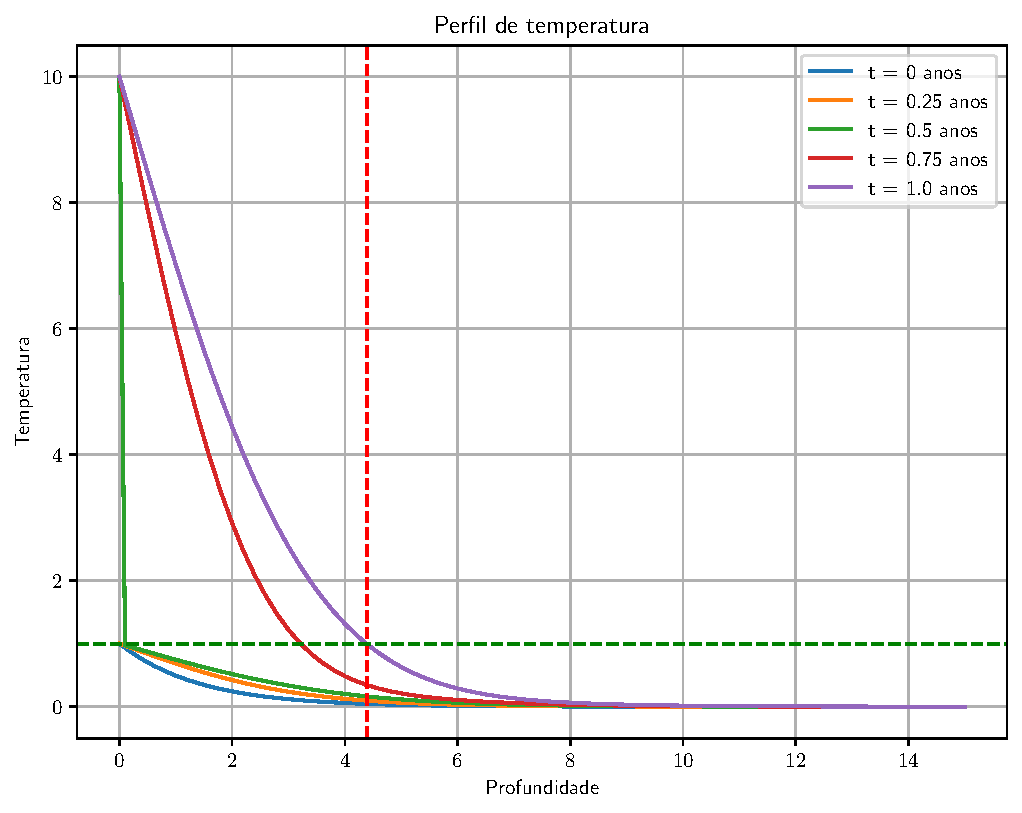
\includegraphics[width=.45\textwidth]{Codes/exp-euler.pdf}
		\caption{Perfil de temperatura para diferentes instantes de tempo calculado usando
		o método de Euler explícito. A reta pontilhada
		vermelha representa a profundidade $x = 4.4$m, enquanto a reta pontilhada verde
		representa a temperatura $y=1$. O perfil de temperatura ao final de 1 ano (curva roxa)
		passa pelo encontro entre as duas retas pontilhadas, mostrando que à profundidade
		de $4.4$m a temperatura tem fase oposta à da superfície.}
	\end{figure}
	%
	A Figura~\ref{fig:exp-euler} exibe o perfil de temperatura em diferentes instantes
	obtidos pelo método de Euler.
	Podemos ver uma mudança abrupta em $t=0.5$, causada pela mudança na condição de contorno
	à esquerda (superfície) de inverno para verão. Na figura também são exibidas as retas 
	$x=4.4$m (em vermelho) e $y=1$ (em verde). Observe que a curva roxa, correspondente
	ao perfil de temperatura ao final de 1 ano, passa pelo encontro das retas, i.e.,
	pelo ponto $(4.4, 1)$. Isso recupera o resultado obtido na análise teórica de que
	à profundidade $4.4$m a temperatura tem fase oposta à temperatura da superfície
	(e, consequentemente, é inverno a essa temperatura enquanto é verão na superfície).
	
	Um vídeo mostrando a evolução do perfil de temperatura pode ser encontrado
	\href{https://github.com/CaioTomas/Trabalho-IMCEDP/blob/main/Report/Codes/exp-euler.mp4}{neste link}.
	%
	\begin{figure}[t]%
		\label{fig:ordem-exp-euler}
		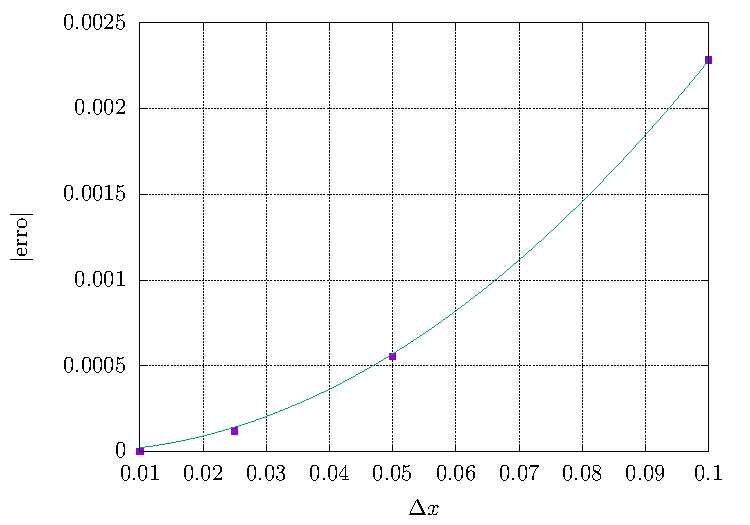
\includegraphics[width=.45\textwidth]{Codes/ordem-exp-euler.pdf}
		\caption{Validação da ordem do método de Euler explícito. Fit da forma $f(x) = ax^2$.
		Erro encontrado de $0.8727\%$.}
	\end{figure}
	%
	Para validar a ordem deste esquema, tomamos como referência o ponto
	$(t_r, x_r) = (1 \text{ ano}, 5 \text{ m})$. Calculamos $T(t_r, x_r)$
	para 4 valores de $\Delta x$: $\Delta x_1 = 0.1$, $\Delta x_2 = 0.05$, $\Delta x_3 = 0.025$
	e $\Delta x_4 = 0.01$. 0 erro foi calculado como $|\Delta x_i - \Delta x_4|$, com $1 \leq i \leq 4$.
	O fit realizado foi do tipo $f(x) = ax^2$ e o erro encontrado no ajuste foi de $0.8727\%$.
	Isto valida a ordem 2 do método.
	
	Também resolvemos o problema usando o método de Crank-Nicolson. Mantemos as mesmas
	escolhas de intervalos, discretização e passos de tempo por simplicidade, mas a estabilidade
	incondicional do método nos fornece uma margem de manobra maior para escolher estes parâmetros.
	%
	\begin{figure}[b]%
		\label{fig:crank-nicolson}
		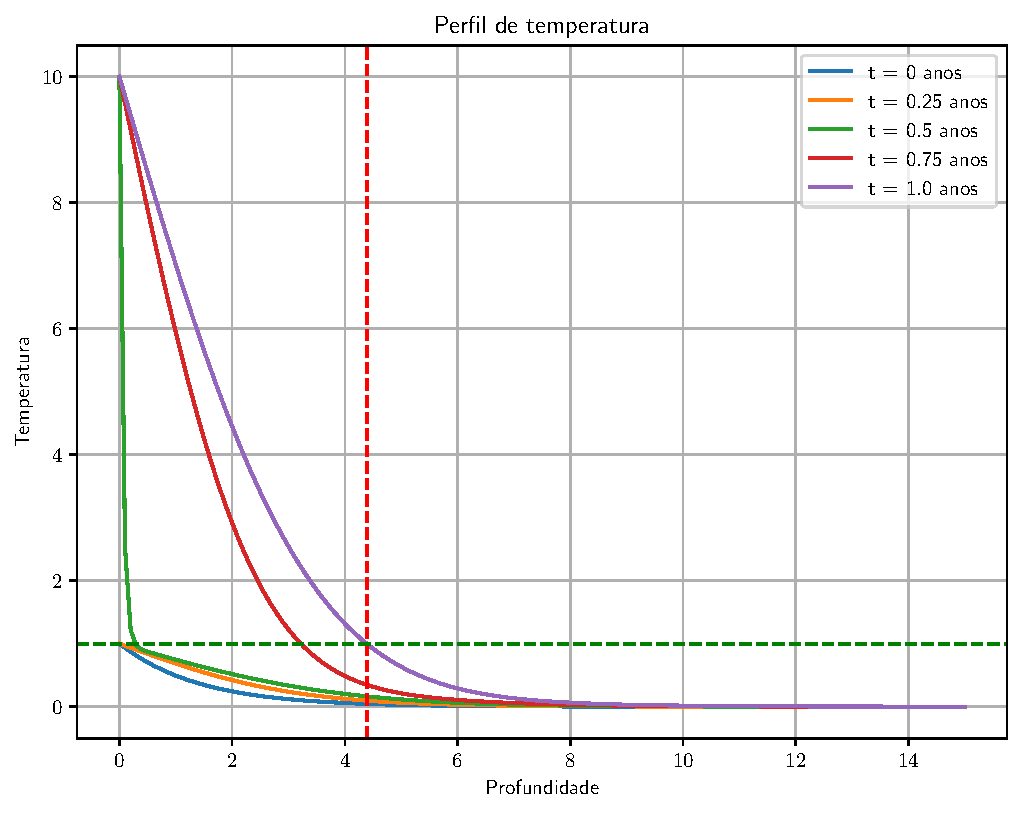
\includegraphics[width=.45\textwidth]{Codes/crank-nicolson.pdf}
		\caption{Perfil de temperatura para diferentes instantes de tempo calculado usando
		o método de Crank-Nicolson. A reta pontilhada
		vermelha representa a profundidade $x = 4.4$m, enquanto a reta pontilhada verde
		representa a temperatura $y=1$. O perfil de temperatura ao final de 1 ano (curva roxa)
		passa pelo encontro entre as duas retas pontilhadas, mostrando que à profundidade
		de $4.4$m a temperatura tem fase oposta à da superfície.}
	\end{figure}
	%
	A implicitude deste método nos obriga a resolver um sistema linear a cada iteração temporal.
	Para tanto, utilizamos o algoritmo de Thomas, próprio para resolver sistemas lineares tridiagonais.
	
	A Figura~\ref{fig:crank-nicolson} exibe o perfil de temperatura em diferentes instantes
	obtidos pelo método de Crank-Nicolson.
	Assim como foi o caso para o método de Euler, podemos ver uma mudança abrupta em $t=0.5$,
	causada pela mudança na condição de contorno
	à esquerda (superfície) de inverno para verão. Na figura também são exibidas as retas 
	$x=4.4$m (em vermelho) e $y=1$ (em verde) e, assim como para o método de Euler, vemos
	que o resultado obtido na análise teórica de que
	à profundidade $4.4$m a temperatura tem fase oposta à temperatura da superfície
	(e, consequentemente, é inverno a essa temperatura enquanto é verão na superfície)
	é recuperado.
	
	Um vídeo mostrando a evolução do perfil de temperatura pode ser encontrado
	\href{https://github.com/CaioTomas/Trabalho-IMCEDP/blob/main/Report/Codes/crank-nicolson.mp4}{neste link}.

	Por fim, consideramos o problema
	%
	\begin{equation}
		u_t = {\left( \kappa(x)u_x \right)}_x,
	\end{equation}
	%
	com $\kappa(x) = {(6.3 + x)}^{\alpha}$ e sujeito às mesmas condições de contorno e condição inicial previamente citadas.
	Dito de outro modo, vamos considerar que a difusividade aumenta com a profundidade
	(quanto mais fundo, mais rapidamente o calor se difunde). Consideramos apenas os casos $\alpha = 1$ e $\alpha = 2$.

	Para integrar esta equação, lançamos mão de um método de volumes finitos: para cada iteração na malha espacial,
	tomamos
	%
	\begin{equation}
		\overline{\kappa}_i = \frac{1}{2}\left( \kappa(x_{i}) + \kappa(x_{i-1}) \right)
	\end{equation}
	%
	e aplicamos o método de Euler com $\overline{\kappa}_i$. Consideramos o mesmo domínio de antes: $0 \leq x \leq 15$ e $0 \leq t \leq 1$.
	Para que o método convergisse, fixamos $\Delta x = 0.1$ e tomamos
	$\Delta t$ suficientemente pequeno para que
	%
	\begin{equation}
		\frac{\Delta t}{\Delta x^2} \leq \frac{1}{2\kappa_{\max}},
	\end{equation}
	%
	com $\kappa_{\max} = {(6.3 + x_{\max})}^{\alpha} = 21.3^{\alpha}$.
	%
	\begin{figure}[t]%
		\label{fig:FVM}
		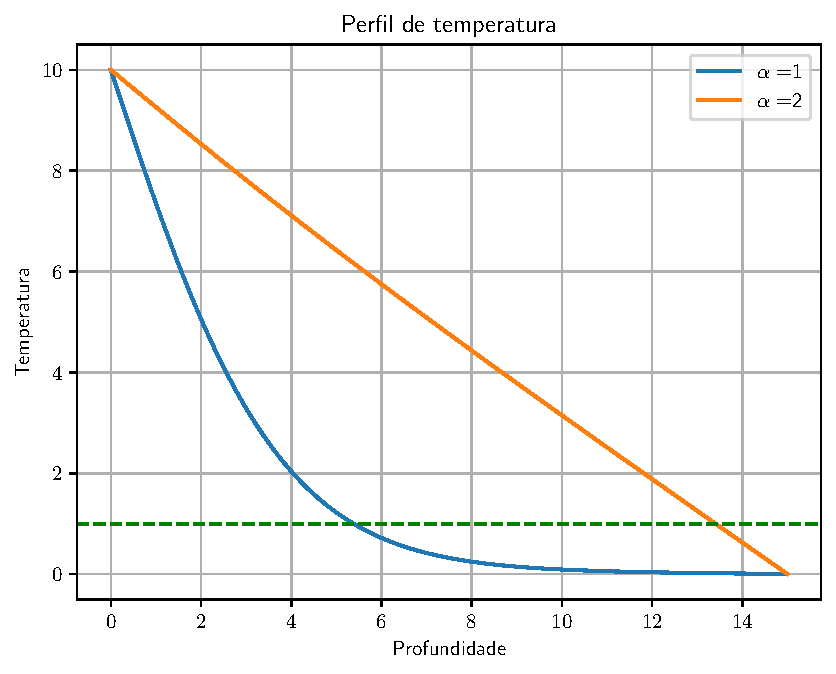
\includegraphics[width=.45\textwidth]{Codes/FVM.pdf}
		\caption{Perfil de temperatura para $t=1$ considerando $\alpha = 1$ e $\alpha = 2$.
		Vemos que a profundidade ideal para a adega aumenta, indo para $x^{\alpha=1} \approx 5.4$m
		e $x^{\alpha=2} \approx 13.4$m.}
	\end{figure}
	%
	A Figura~\ref{fig:FVM} traz os perfis de temperatura para $\alpha=1$ (azul)
	e $\alpha = 2$ (laranja) ao final de 1 ano. A reta verde pontilhada marca a temperatura da superfície no inverno.
	Vemos que a profundidade ideal para a adega aumenta, indo para $x^{\alpha=1} \approx 5.4$m
	e $x^{\alpha=2} \approx 13.4$m.
%
\section{Códigos utilizados}
%
	Este projeto pode ser encontrado
	\href{https://github.com/CaioTomas/Trabalho-IMCEDP}{neste link},
	incluindo os códigos utilizados para o cômputo da solução e o código-fonte
	deste documento.


% \printbibliography
% \bibliography{Report/referencias}

\begin{thebibliography}{9}
	\bibitem{Iserles} Arieh Iserles, \textbf{Cambridge Texts in Applied Mathematics}: \textit{A First Course in the Numerical Analysis of Differential Equations}, 2nd edition (Cambridge University Press, 2008)
	\bibitem{lin1998} C.C. Lin, L.A. Segel, \textbf{Classics in Applied Mathematics 1}: \textit{Mathematics Applied to Deterministic Problems in the Natural Sciences}, (Society for Industrial and Applied Mathematics, 1998)
\end{thebibliography}

\appendix

%
\section{O método de Thomas para solução de sistemas tridiagonais}
%
	Seja
	%
	\begin{equation}
		\begin{bmatrix}
			b_1 & c_1 &     &        &  \\
			a_2 & b_2 & c_2 &        &  \\
			    & a_3 & b_3 & \ddots &  \\
			    &     & \ddots & \ddots & c_{n-1} \\
			    &     &  & a_n & b_n 
		\end{bmatrix}\begin{bmatrix}
			x_1 \\
			x_2 \\
			x_3 \\
			\vdots \\
			x_n
		\end{bmatrix} = \begin{bmatrix}
			d_1 \\
			d_2 \\
			d_3 \\
			\vdots \\
			d_n
		\end{bmatrix}
	\end{equation}
	%
	um sistema linear tridiagonal. O método de Thomas é um método que resolve tais sistemas em $\mathcal{O}(n)$
	operações\footnote{Compare com as $\mathcal{O}(n^3)$ operações necessárias para a eliminação gaussiana.},
	realizando uma primeira varredura para eliminar os $a_i$'s seguida de uma substituição inversa.
	Este algoritmo não é estável para o caso geral. Não obstante, o método de Crank-Nicolson nos dá $b_i = 1 + 2\alpha$,
	$a_i = c_i = -\alpha$ e, neste caso, a matriz do sistema é estritamente diagonalmente dominante e o algoritmo é estável.

	A primeira etapa do método consiste de uma varredura para o cômputo de novos coeficientes $c_i'$ e $d_i'$ dados por
	%
	\begin{equation}
		c_i' = \begin{cases}
			\displaystyle{\frac{c_i}{b_i}}, \ i = 1 \\
			\displaystyle{\frac{c_i}{b_i - a_i c_{i-1}'}}, \ 2 \leq i \leq n-1
		\end{cases}
	\end{equation}
	%
	e
	%
	\begin{equation}
		d_i' = \begin{cases}
			\displaystyle{\frac{d_i}{b_i}}, \ i = 1 \\
			\displaystyle{\frac{d_i - a_i d_{i-1}'}{b_i - a_i c_{i-1}'}}, \ 2 \leq i \leq n
		\end{cases}
	\end{equation}
	%
	Calculados os novos coeficientes, a solução é dada por
	%
	\begin{align*}
		x_n &= d_n' \\
		x_i &= d_i' - c_i' x_{i+1}, \ i = n-1, n-2, \dots, 1.
	\end{align*}
	%

\end{document}